\chapter{Methodology}\label{chap2}
\thispagestyle{plain}

%This chapter provides a detailed description of the methodology. It is
%sometimes called Experimental Section. Depending on the subject it is a
%``synonym'', e.g., for Theoretical Section, Computational Methods, Model
%Description and Setup, Field Work, and so on. Hence, this chapter contains a
%description of \emph{what has been done} in order to address the scientific
%question raised in the chapter Introduction. However, it does \emph{not} contain
%the results! 


% ==== SECTION 1 ===============================================================
%\section{Experimental Set-up}\label{2sec:1}
%Depending on the topic of the science thesis, this chapter may contain a
%description of the experimental set-up, the field experiment,
%datasets, instruments, measurement procedures, analysis techniques, calibration
%and quality control, and other things. In case of a modeling study it may
%contain the formulation and derivation of model equations, the formulation of
%initial and boundary conditions, the data used to drive and validate the model,
%an overview of the model set-up (e.g., parameter set-up), modifications of the
%``original'' model code, a description of relevant parameterizations,
%a theoretical background needed for the interpretation of model results.


% ==== SECTION 2 ===============================================================
\section{Data Sets}\label{glathida}
This section gives an overview of the data used in the analysis done in this thesis. The basics data to run all the analysis have been the Glacier Thickness Database (GlaThiDa), the Randolph Glacier Inventory (RGI), and different digital elevation models (DEMs) which are dependent on the specific glacier. Depending on the region in fact some digital elevation models are a better fit to each glaciers as all of the freely available ones have missing data. ``The best'' digital elevation model has been automatically chosen by the Open Global Glacier Model (OGGM). Through most of the analysis SRTM v4 (\citet{SRTM}) which is a 90m grid resolution DEM has been used. Other DEM might have been used to link the GlaThiDa with RGI (see section \ref{GlaRGI})

\subsection{GlaThiDa}
The glacier Thickness Database (\citet{GlaThiDa2014}) is a set of data which attempts to put together all the available ice thickness measurements from glaciers and ice caps all around the globe. The database is composed of three different tables. The first one contains an overview of the database, the second one thickness data from maps or digital elevation models (DEM), and the third one, the one used in this thesis, contains the actual point measurements with the thickness data. The measurements were taken with different methods such as terrestrial and airborne radio-echo sounding, ground penetrating radar, direct drilling and other methods. The first database was released in 2014. In 2016 a second version 2.0 and its correction 2.1 were released, and in 2019 version 3.0 and 3.01 were finally released. All the analysis in this work have been done using version 2.1 as version 3.0 was released after a big part of the analysis was already done. According to the \href{https://github.com/ezwelty/glathida/blob/master/CHANGELOG.md}{change log} however most of the changes have been done to the structure of the data base. There were however some measurements additions to the database. The addition of some measurements for some glaciers in Switzerland in particular would be relevant for this thesis, given that most of the analysis done in this work has been conducted over the alpine glaciers. 
%Use subsections to structure your thesis. The first and second component of the
%momentum equation is shown in equation (\ref{2equ:1}) and (\ref{2equ:2}),
%respectively. Together with (\ref{2equ:3}) they form the set of shallow-water
%equations implemented in a numerical model.

\subsection{RGI}
The Randolph Glacier Inventory (RGI) (\citet{RGI2014}) is a global database of outlines of glaciers, excluding ice sheets. The inventory has been compiled from satellite imagery collected from 1999 onward. Most of the outlines don't express a specific picture in time of the glacier but are a compound of different images of each glacier due to images obstructions such as cloud covers or satellite orbits. The first version of this inventory was released in 2012 and the latest version, RGI Version 6.0 was released in 2017. In this latest release the database comprises more than 220,000 glacier outlines which are divided in 19 regions which cover all areas in the world with glaciers. This is the version used for all the analysis in this thesis. \todo{Add map of all the glaciers?}

\subsection{Linking GlaThiDa and RGI}\label{GlaRGI}
The GlaThiDa comes with a table containing the thickness measurements observations. This table comes with the thickness value of the observation, its latitude and longitude, and other variables such as the date of the observation, the name of the glacier, the thickness uncertainty and others. Aside from the measurements GPS coordinates and the thickness value, some fields like, the name of the glacier and the thickness uncertainty, are often left empty. This creates the problem of having to link each observation with a glacier in the RGI database. To do so a script has been created which determines whether an observation is located inside a glacier outline: the RGI database comes with closed outlines of the glaciers in geographic coordinates referenced to the WSG84 (also known as ESPG:4326) as shape-files. The python library \href{https://github.com/Toblerity/Shapely}{shapely} has been used to transform the observation Latitude and Longitude to the WSG84 projection system and to check whether each of these point was lying inside the glacier outlines (including the boundaries of the outline).
\todo{Add graphic of a glacier with the thickness points. I couldn't find a script with it so far.}

\subsection{Some statistics about GlaThiDa}
After linking the two databases it is interesting to learn about some statistics of the GlaThiDa. In order to create these statistics The Open Global Glacier Model (OGGM) (\citet{OGGM2019}, \href{https://github.com/OGGM/oggm}{Open Source Code}) has been used to add a digital elevation model to the glaciers in the RGI with thickness entries in the GlaThiDa (see \ref{GlaRGI}).

\subsubsection{Glaciers distribution and types}
There are 820370 entries (thickness measurements) in the GlaThiDa version 2.1. After assigning each of them to one of the 215,547 RGI glaciers 771 of those glaciers have thickness observations associated with them. This is 0.36\% of all the glaciers in th RGI. Out of the 820370 initial entries 27882, 3.4\% resulted outside of any glacier outlines defined in the RGI. Some reason for this could be: a slightly wrong GPS coordinate collected in the GlaThiDa measurement; observations taken outside of the glacier by mistake or intentionally, to make sure that all the glacier was covered; a different shape of the glacier at the moment when the observation was taken, compared to the moment when the RGI was compiled; a wrong assessment of the glacier shape in the RGI.
\begin{figure}\label{glathidamap} 
	\centering 
	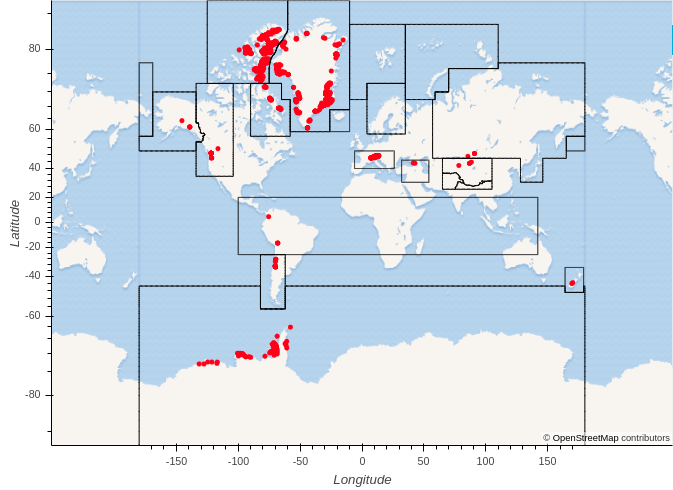
\includegraphics[width=1.0\textwidth]{./figures/GlaThiDa_map.png}
	\caption{Global map of the distribution of glaciers with thickness observations entries in the GlaThiDa database version 2.1. Black outlines are the RGI regions.}
\end{figure}

Most of the glaciers with thickness observation are in the Greenland Periphery region and in the Artic Canada North region. If we compare the glaciers with measurements with the number of glaciers present in each specific region though, we see that Arctic Canada North is the best represented region with around 5\% of the glaciers having at least one thickness measurement point. The region with most glaciers, Central Asia, has a very low number of glaciers represented in the GlaThiDa database. This is probably due to the difficulty in getting measurements for glaciers as such high altitudes at those present in the Himalaya.


\begin{figure}[!tp]
	\centering		  
	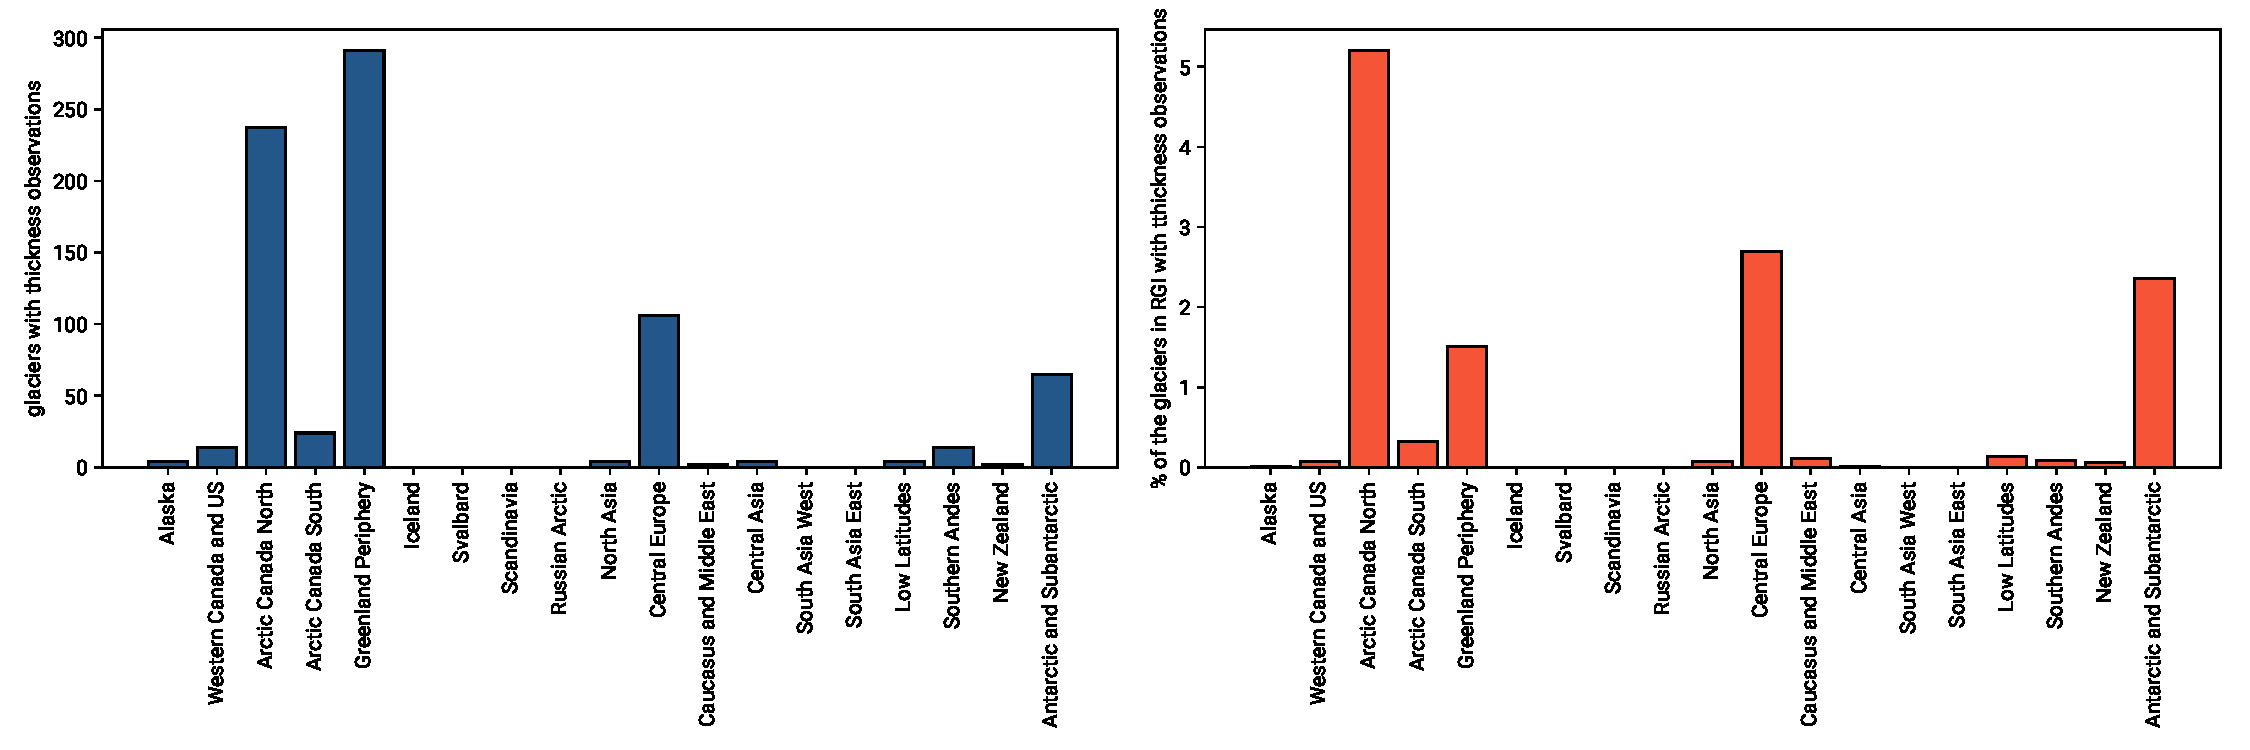
\includegraphics[width=1.\textwidth]{figures/Observations_per_region.pdf}
	\caption{On the left side the number of glaciers in the RGI with thickness observations in the GlaThiDa are shown per RGI region. On the right side the percentage of glaciers for each region with thickness observations is shown instead.}
	\label{fig:glareg}
\end{figure}

More than two third of the RGI entities with GlaThiDa measurements are glaciers while the rest are ice caps. Land terminating glaciers and ice caps are the vast majority.

\subsubsection{Measurements Distribution per Glacier}
Not all the glaciers with measurements are perfectly covered over the whole glacier area. In fact around 42\% of the glaciers have less than 100 thickness observations. Given that some glaciers can extend for over $100 km^2$, it’s clear that some of them are very poorly covered.
\begin{figure}[!tp]
	\centering		  
	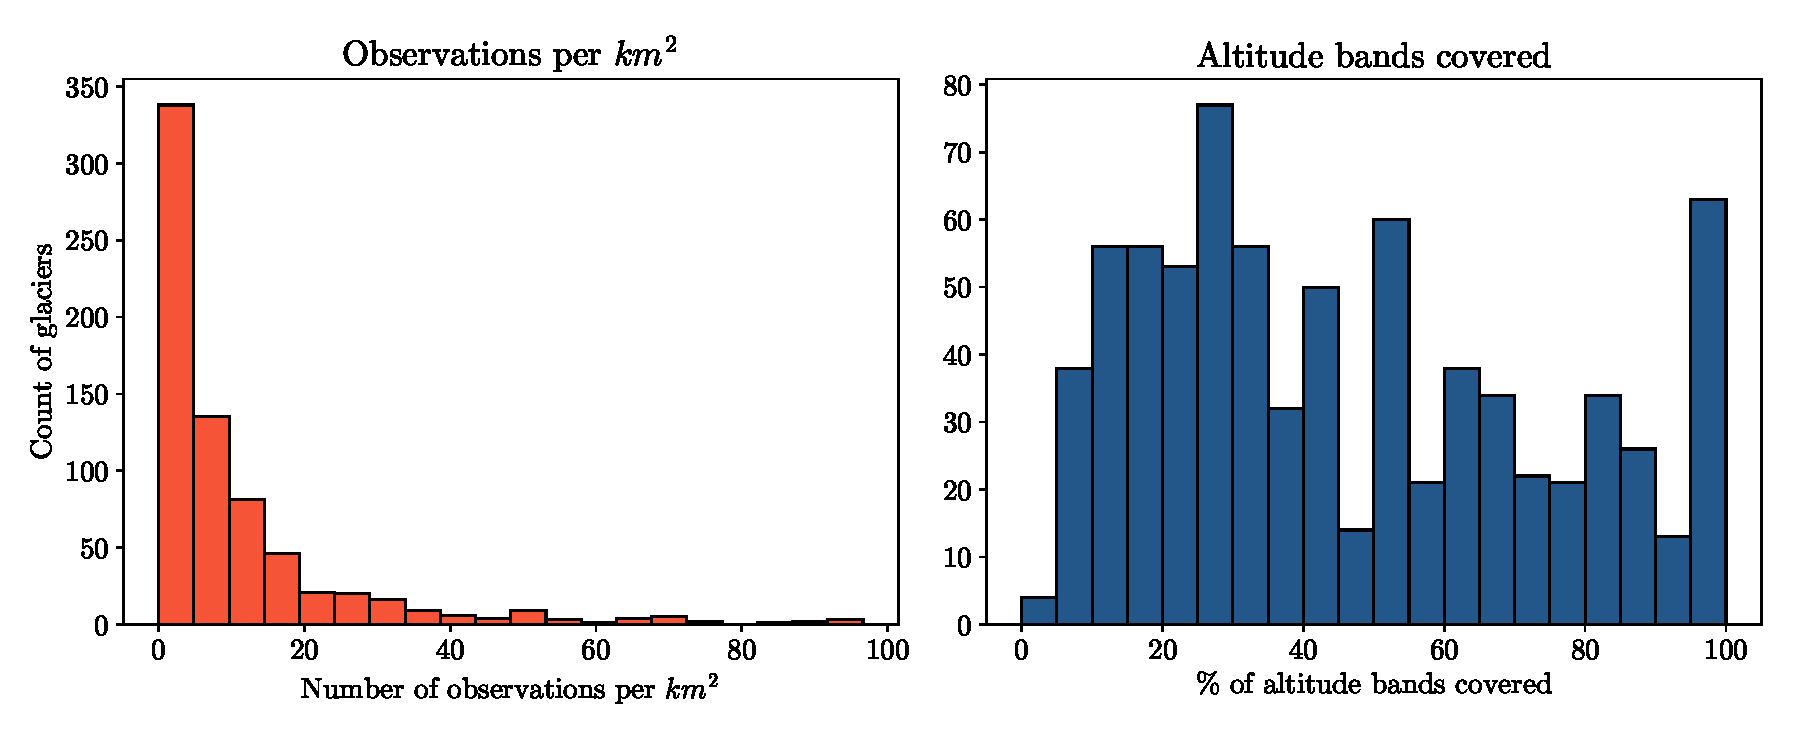
\includegraphics[width=1.\textwidth]{figures/Observations_per_skm.pdf}
	\caption{On the Left: distribution of glaciers with less than 100 observations per squared kilometer; there is a great number of glaciers with less than 20 thickness observations per squared kilometer. On the right: distribution of glaciers according to the percentage of their altitude bands covered.}
	\label{fig:glaobs}
\end{figure}

More than 91\% of all the glaciers (represented in the figure above) have less than 100 thickness measurements per squared kilometer. Almost 44\% of all the glaciers with thickness observations have less than 5 observations per squared kilometer (see Fig. \ref{fig:glaobs}).

OGGM was used to generate a gridded map of each glacier represented in the GlaThiDa. With this map one can divide each glacier in $100m$ altitude bands to check how many of those bands contain at least one thickness measurement.
Almost half of the glaciers have observations in at least half of the 100m altitude bands (see Fig. \ref{fig:glaobs}). Glaciers with few observations but well distributed over their length can be very useful for understanding glacier thickness patterns and for model validation.

\subsubsection{Survey Year}
Measurements were taken between 1977 and 2015, but most of them after 2005 (see Fig. \ref{fig:glayears}). The spread in the dates of the campaigns for taking the observations could potentially create problems when trying to compare glaciers with each other to find similar patterns, but also when using the data for model validation.
Most glacier models make in fact use of digital elevation models to setup the model run. Any digital elevation model is compiled with data available at the time of its construction. The time difference between the date of data assimilation for the digital elevation model, and the date of the survey for the thickness observation, could be in the order of several years. This would create an error when validating the model.
\begin{figure}[!tp]
	\centering		  
	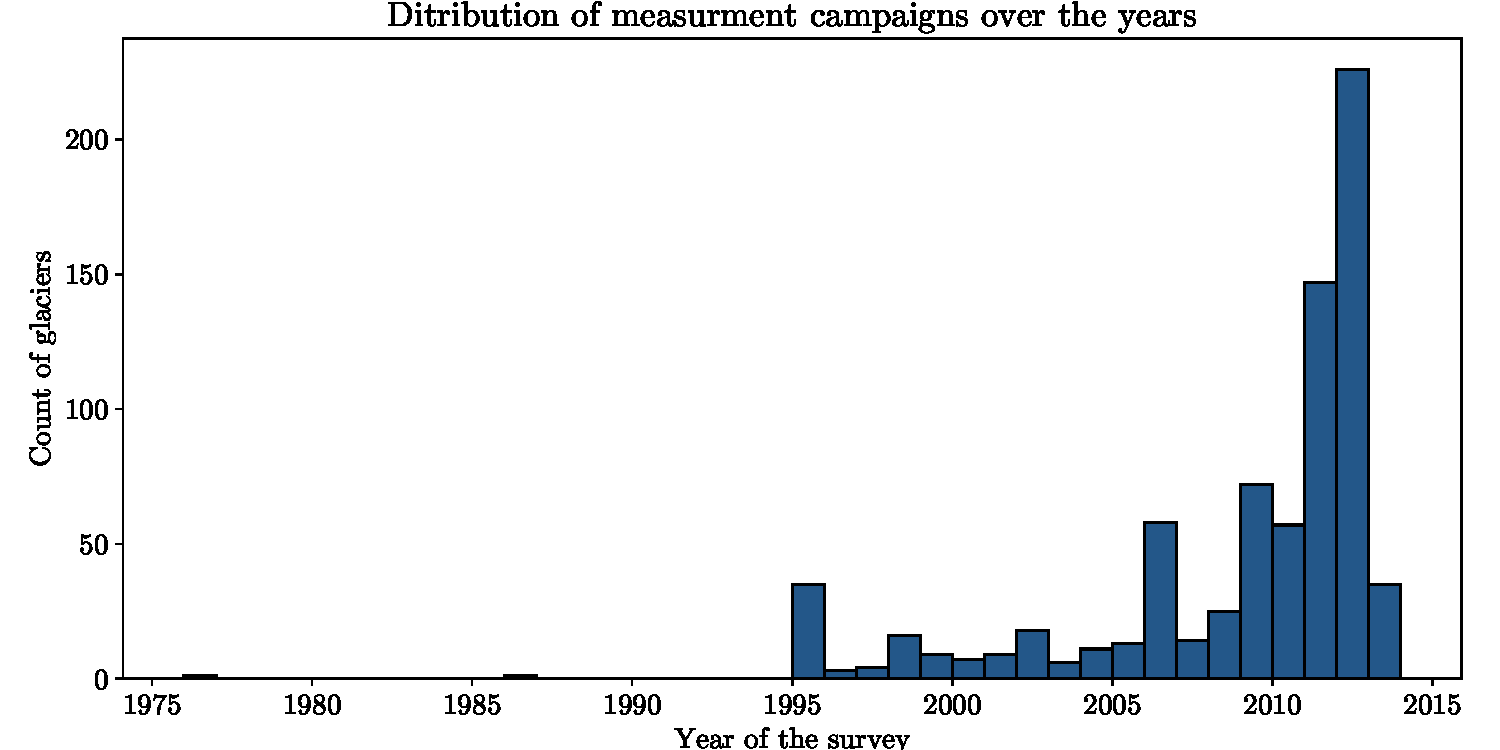
\includegraphics[width=1.\textwidth]{figures/Observations_per_year.pdf}
	\caption{Distribution of glaciers with observations in the GlaThiDa according to the year when the measurements for each glacier were taken.}
	\label{fig:glayears}
\end{figure}


\section{Machine Learning Algorithms}\label{ML}
Machine learning is a mathematical method which enables computers to perform a specific task without giving it the specific instructions on how to do it. This is achieved using algorithms to build a model from data usually called the ``training data''. This data are given to the algorithm which uses an iterative process to create the final model. 

The idea behind it is to emulate the learning process of a human-being in order to make predictions about new data. If for example one wanted to teach a kid how to recognize a cat, the simpler approach would be to show it cats or pictures of them, instead of trying to explain it what are the key attributes which characterize cats. In the same way machine learning algorithm are used to make predictions without giving them instructions (explaining the key characteristics) about how to do the predictions, but rather by feeding them examples.

The branch of machine learning used in this thesis is called ``supervised learning'' which builds models learning from data which contain the input variables and the desired output value, often refereed to as labels.
The machine learning algorithm is then used to find the target function $f$ which better maps input vector $X$ to an output one $Y$.
\begin{equation}
Y = f(X)
\end{equation}
The way this function is computed by the algorithm depends on the specific one chosen to achieve the desired result.

In this thesis three different machine learning algorithm have been used to train models which estimate the ice thickness of glaciers using the GlaThiDa database as the desired output ($Y$) for the ice thickness, and using digital elevation models and some basic physics assumptions as the input values ($X$), to obtain the ice thickness distribution of the glacier.

The three algorithm used are:
\begin{itemize}
	\item Linear Regression
	\item Random Forest Regression
	\item Support Vector Regression (SVR)
\end{itemize}

The algorithms have been applied to the data using the python package \href{https://scikit-learn.org/}{scikit learn}.
%The way the algorithm achieves this without instructions from the programmer is with an iterative process which uses the training data to make a first prediction, compare the prediction with the the desired output value, 
\subsection{Linear Regression}
Linear Regression is probably one of the simplest machine learning algorithm and also one of the most used (even though many people probably don't know it is a machine learning algorithm).

Given a set of input data $\bm{X} = \{x_{i1},\ldots ,x_{ip}\}_{i=1}^{n}$ and a corresponding output $\mathbf{y} = \{y_{1},\ldots ,y_{n}\}$, the algorithm finds the best set of $\bm{\beta} = \{\beta_{i1},\ldots ,\beta_{ip}\}_{i=1}^{n}$ and $\bm{\varepsilon} = \{\varepsilon_{1},\ldots ,\varepsilon_{n}\}$ such that:
\begin{equation}\label{eq:linear}
\mathbf {y} = \bm{\varepsilon} + \bm{\beta}\bm{X}
\end{equation}
In order to find $\bm{\varepsilon}$ and $\bm{\beta}$ which best predict the desired $\mathbf {y}$, one of the most common approaches is to minimize the loss function
\begin{equation}
\frac{1}{n}\sum_{1}^{n}(pred_i-y_i)^2
\end{equation}
where $pred_i$ is the value of the $i$-th prediction generated by the model.

This algorithm is clearly only useful for cases when the output variables linearly depend on the input ones. This is however often not the case thus requiring most sophisticated models to compute the desired output values. It can be helpful however to compare this method to the more sophisticated ones to have a basic reference on their performances.

\subsection{Random Forest}
\begin{figure}[!tp]
	\centering		  
	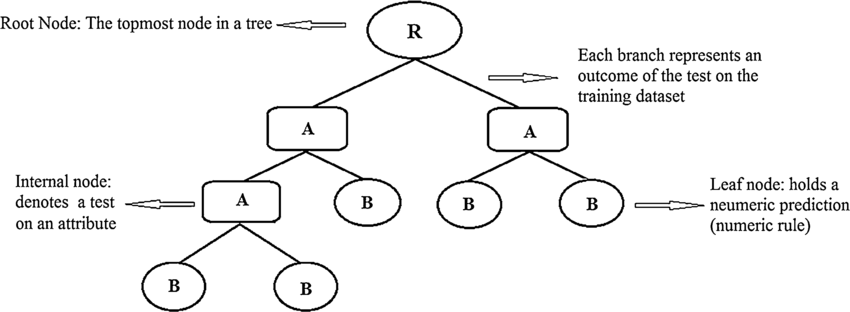
\includegraphics[width=1.\textwidth]{figures/decision_tree.png}
	\caption{Representation of a decision tree model. The tree is pictured upside-down with the root on the top and the branches and leaves on the bottom.}
	\label{fig:tree}
\end{figure}
Random Forest is an algorithm which uses ensemble learning to extend and improve the performances of decision trees algorithm. The method was first proposed by \citet{RandomHo1995}. A decision tree is an algorithm used to predict the desired value from a set of data. It works by splitting the data-set into a number of branches by imposing conditions on each feature. Every split leads to a subset of the data-set which can be split further to better achieve the desired outcome(see \ref{fig:tree}). In order to choose how to split the data on each node the algorithm calculates the sum of the squared residual for splitting the data-set on a particular condition and chooses the condition which minimizes this sum. Let $\bm{X} = \{x_{i1},\ldots ,x_{ip}\}_{i=1}^{n}$ be the $n$-th input values $p$ the different attributes  our data-set and $\mathbf{y} = \{y_{1},\ldots ,y_{n}\}$ the output values (the values we want to predict). Let's assume for simplicity that we are splitting the data based on a condition on the first attribute. The first split in the tree divides the data-set into two subsets $S_1$ with $l$ data points and $S_2$ with $n-l$ data points. The subsets are defined so that the following is minimized:
\begin{equation}\label{eq:treeres}
\sum_{i \in S_1}(\overline{y_1}-y_i)^2 + \sum_{j \in S_2}(\overline{y_2}-y_j)^2
\end{equation}
where  $\overline{y_1} = \frac{1}{l}\sum_{i \in S_1}y_i$ and $\overline{y_2} = \frac{1}{n-l}\sum_{j \in S_2}y_j$. The method can then be repeated to create further branches and a deeper tree. In order to choose which feature to use as a condition for the split, \ref{eq:treeres} is calculated for each feature and the one resulting in the minimum value draws the condition for the split on the node. The algorithm usually stops when the minimum arbitrary number of observations for each subset is reached.

The problem with decision trees is that they are inaccurate for predictions with data outside the ones used to create them (\cite{hastie01statisticallearning}).
To solve this problem Random Forest algorithm relay on an ensemble of decision trees to make the predictions. Each tree in the ensemble (forest) is constructed using the same number of input values $n$, but randomly selecting the input values with replacement: each input value can be chosen more then once to be part of the sample constructing the three, leaving out some of the input values from this sample. In addition to this, each tree is only limited to a subset of features to choose from to split the data at each node. After each tree is trained the prediction is made by averaging the predictions from al the trees in the forest. Additionally an estimate of the uncertainty of the prediction can be calculated from the standard deviation of the predictions from all the trees.



\subsection{Support Vector Regression}
Support Vector Regression (SVR) was first presented as regression extension of the support vector machine algorithm (SVM) by \citet{SVR1997}. Support vector machine is a supervised machine learning algorithm for classification (i.e. the desired output has binary values) first proposed by \citet{SVM1964}.

Let's assume a training data-set of $n$ points ${({\mathbf {x}}_{1},y_{1}),\ldots ,({\mathbf {x}}_{n},y_{n}),}$, where $y_{i}$ are either $1$ or -$1$, each indicating a different class, the value we want to predict, for the points ${\mathbf {x}}_{i}$. Each ${\mathbf {x}_{i}}$ is a $p$-dimensional real vector. We want to find the decision boundary that divides the group of points $\mathbf {x}_{i}$ for which $y_{i}=1$ from the group of those for which $y_{i}=-1$. This boundary is defined in such a way that the distance between the hyperplane and the closest ${\mathbf {x}}_{i}$ from either group is maximized.
An hyperplane is defined as the points ${\mathbf {x}}$ satisfying 
\begin{equation}\label{eq:svm}
\mathbf {w}\cdot \mathbf {x}-b=0
\end{equation}

where $\mathbf {w}$ is the normal vector to the plane. $b$ determines the offset of the hyperplane from the origin.

If the training data were linearly separable two parallel hyperplanes must exist separating the two classes of data points such that the distance between the two is maximized. The equations for these planes are respectively:

\begin{align}
\label{eq:planes1}
	\begin{split}
	\mathbf {w}\cdot \mathbf {x}-b = 1, \\
	\mathbf {w}\cdot \mathbf {x}-b = -1
	\end{split}
\end{align}

These two hyperplanes would determine the margin between the two groups. The data points ${\mathbf {x}}_{i}$ lying nearest to these two hyperplanes are called the support vectors. The hyperplane lying exactly in the middle of the two is called decision boundary. This hyperplane separates the two groups of data. If one wanted to label a new data point not used to train the model, this point would be classified depending on which side of the decision boundary it would lie on. This is called a hard margin.

\begin{figure}[!tp]
	\centering		  
	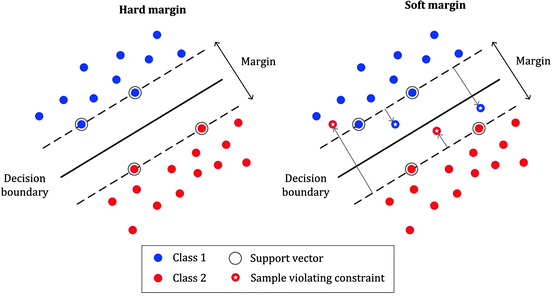
\includegraphics[width=1.\textwidth]{figures/SVM.png}
	\caption{Representation of support vector machine in a 2-dimensional space. On the left a model is trained with the creation of an hard-margin which correctly classifies each sample in the training data-set. On the right a soft-margin is selected which allows a number of miss-classified points to lie inside the margin.}
	\label{fig:svm}
\end{figure}

The distance between the two plains is ${\frac {2}{\|{\mathbf {w}}\|}}$. In order to maximize this distance we then need to minimize $\|{\mathbf {w}}\|$, with the constrain

\begin{equation}\label{eq:svmconstrain}
y_{i}({\mathbf {w}}\cdot {\mathbf {x}}_{i}-b)\geq 1
\end{equation}
for all $i=1,\ldots ,n$ given by the fact that each point must lie outside the margin (see Eq. \ref{eq:svrconstrain}).

This algorithm works well for linearly separable data-sets. If however the data were non linearly separable, or if outliers or miss-classifications were included in the data-set, as in most real  world cases, one would instead choose a so called "soft-margin" which would work exactly like the hard margin but with allowance for a number of miss-classified data points (see Fig. \ref{fig:svm})

To extend this concept for a regression case, i.e. a case where the output values $y_{i}$ are continuous, we can use the same concept with but with the objective of finding a function $f(x)$ which deviates from each $y_{i}$ by a value not greater than $\varepsilon$ and is as flat as possible.

\begin{equation}\label{eq:svr}
f(x) = \mathbf {w}\cdot \mathbf {x}-b
\end{equation}

This would mean to minimize $\|{\mathbf {w}}\|$ subject to the constrain:

\begin{equation}\label{eq:svrconstrain}
|y_{i} - {\mathbf {w}}\cdot {\mathbf {x}}_{i}+b|\leq \varepsilon
\end{equation}
for all $i=1,\ldots ,n$.

To extend the algorithm to non linear cases SVM and SVR apply the so called "kernel trick". The algorithm is applied in a transformed higher dimensional space. The resulting boundary hyperplane is linear in the transformed space but might be non linear in the original space.
There are different ways, called kernels, to transform the space to a higher dimensional one. Some of the most common ones, and the ones available in the package \href{https://scikit-learn.org/}{scikit learn} used for the analysis in this thesis, are:
\begin{itemize}
	\item Polynomial
	\item Radial Basis Function
	\item Sigmoid
\end{itemize} 

The one chosen for the analysis in this thesis is the Radial Basis Function kernel (rbf) which transforms the space like so:
\begin{equation}\label{eq:rbf}
k({\mathbf {x_{i}}},{\mathbf {x_{j}}})=\exp(-\gamma \|\mathbf {x_{i}}-\mathbf {x_{j}}\|^{2})
\end{equation}
for $\gamma >0$.
The algorithm basically adds dimensions which are dependent on the distance between the data points. Points with higher distances are less influenced by each other because of the exponential decay which relates the distances.

The kernel trick and is what makes support vector regression so powerful because it allows the algorithm to learn from non linear relationship between the data.

\begin{figure}[!tp]
	\centering		  
	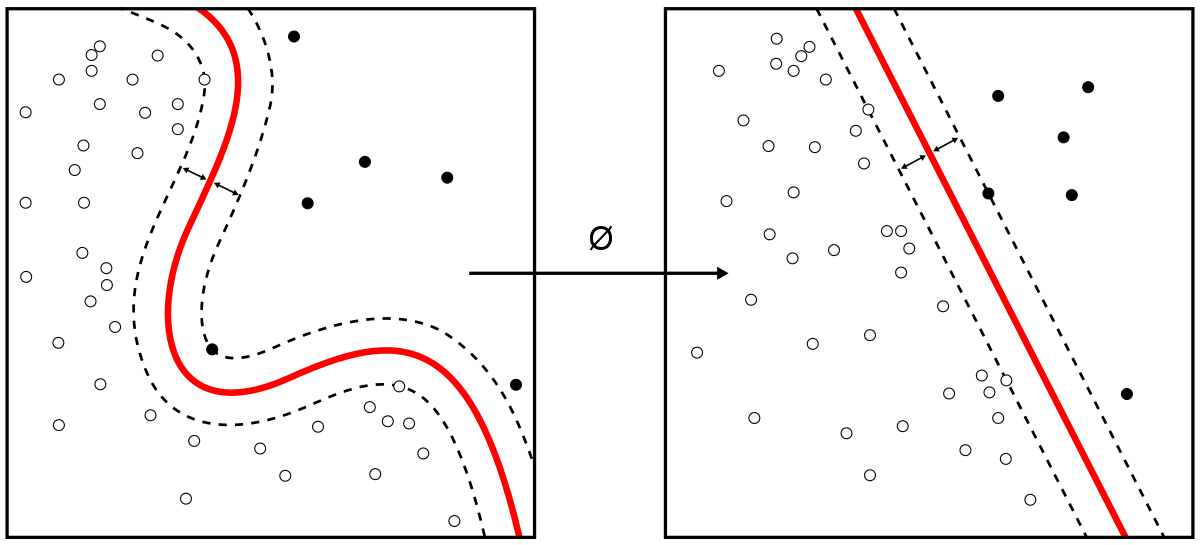
\includegraphics[width=1.\textwidth]{figures/kernel_trick.png}
	\caption{Representation of the kernel trick: the initial 2-dimensional space on the left gets transformed into a 3-dimensional one on the right by the kernel function. An hyperplane can be fit in the new 3-dimensional space to correctly separate the data with a linear decision boundary.}
	\label{fig:kernel}
\end{figure}

\subsection{Tuning parameters}
How did we decide which parameters to use (maybe we can just leave it for the appendix)

\section{Training method}\label{training}
In order to train the model one needs to feed the chosen machine learning algorithm a training data-set. One could simply take all the data from the set and feed the to the algorithm. The trained model would then be able to make predictions on a new set of data for which we are lacking labels. In this specific case one could take the input parameters chosen to train the model with, from glaciers for which we are lacking thickness measurements, and predict the thickness for those glaciers. Even more simplistically one could obtain the whole ice thickness distribution for glaciers where we do have thickness measurements, just because these measurements never cover the whole glacier surface. In this way one could extrapolate the thickness distribution of the glacier from the trained model.

The problem with the approach of using all the labeled data available for training however, is the risk of over-fitting the model and the fact that there is no way of assessing the model performances for glaciers without thickness measurements available.
Over-fitting in machine learning means to train a model which is very good at labeling data which were used for training the model, but not able to generalize the results for making predictions about new data. This would lead to a model which is very capable of predicting ice thicknesses for data points which were fed to the algorithm to train the model, but wouldn't be able to make correct predictions for data outside the ones used for the training process. 

In order to avoid over fitting and to be able to have data to asses the performance of the trained model, only part of the available data from the GlaThiDa database was fed to the algorithms to train the models. In particular 75\% of the data were used for training the model and 25\% for assessing performance on new data. This process was achieved with a function available form the python package \href{https://scikit-learn.org/}{scikit learn} which shuffles the data and then randomly picks the data points used for training. The algorithm actually uses a pseudo-random generator to pick the data which one can fix in order to always  have the same data picked by the algorithm when dividing them for training and testing. This process was then repeated 20 times to be able to compare the model performances subject to training with different data. This should improve the ability of generalization for the trained model (\citet{crossval1995}).

\section{Scoring method}\label{scoring}
Once the the model is trained with the training subset of data as described in section \ref{training}, it is important to choose a way to assess the performance of the model. To do this the score method from \href{https://scikit-learn.org/}{scikit learn} has been used on all the models. Let assume the testing input data to consist of $n$ points. Let $y_i$ be the $i$-th prediction done by the model for the $\mathbf{x_i}$ input value of this $n$ points. Let $y^*_i$ be the $i$-th ``true'' label for the $\mathbf{x_i}$ input value and $\overline{y^*}$ the mean value for these true labels (i.e. $y^*_i$ is the thickness value from the GlaThiDa database). The score is then defined as:

\begin{equation}\label{eq:score}
R^2 = 1 - \frac{\sum_{i}^{n}(y^*_i-y_i)^2}{\sum_{i}^{n}(y^*_i-\overline{y^*})^2}
\end{equation}

The best possible score is $R^2 = 1$ and it can be negative (because the model can be arbitrarily worse). A model always predicting the same constant value of $y$ independently on the input values would get a $R^2 = 0$. Note that the $R^2$ score can be negative in case the model performance were worse than a model with constant output $y$.

\section{Features Importance}\label{featuresimp}
Aside for making predictions trained machine learning models can be used to gather information about the importance of each feature in the training data-set. In other words it is possible to get information about which of the features have the most influence when making a prediction. This can be interesting to understand the physical processes driving the ice thickness distribution.

In a linear model this could be easily done my looking at the the magnitude of the coefficients of the linear equation \ref{eq:linear}. In other words one would look at the values of the components of the $\mathbf{w}$ vector. The higher the magnitude the more influential is that feature on making prediction.
However for more complex models like the Support Vector Regression and Random Forest Regression it is not possible to obtain these values because the relationship between the input values and the predicted ones is non-linear. This would actually be possible in the case of a Support Vector Regression using a linear kernel but the space transformation applied by non linear kernel trick makes this impossible.

To solve the aforementioned problem and gather information about the importance of the features two alternative methods have been used:
\begin{itemize}
	\item Permutation Importance
	\item Partial Dependence plots
\end{itemize} 

\subsection{Permutation Importance}

\begin{figure}[!tp]
	\centering		  
	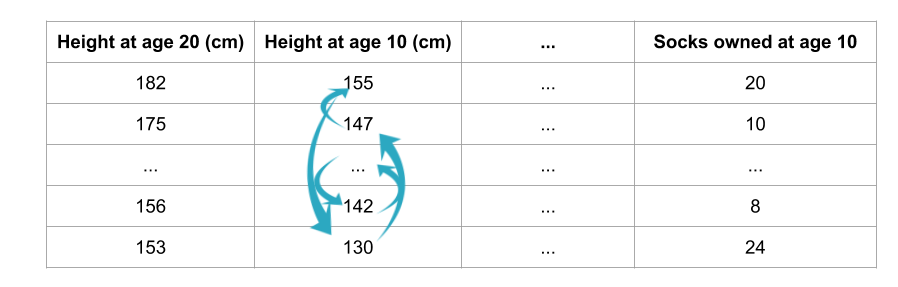
\includegraphics[width=1.\textwidth]{figures/permutation.png}
	\caption{Representation of shuffling the data for a sample data-set. Input values for one features are shuffled randomly switching the data with each other. The score of the model computed with this permuted data is computed and is compared  to the score the model would have for the non-permuted feature.}
	\label{fig:permutation}
\end{figure}

Permutation importance is a simple yet effective way of getting information about which feature drives the outcome in the predictions. To use this method one needs to split the data into two group, one for training and one for testing as reported in section \ref{training}. The method works by training the model as usual. After training is completed the accuracy of the model is tested using the sample left out from the training process. Instead of using the validation inputs as they are in though, the input values from one of the features get randomly shuffled. In this way for example for the selected feature the $i$-th input value corresponding to the $i$-th label gets switched with the $j$-th one corresponding to the $j$-th output one. Now when trained the model will get the $j$-th input value for the $i$-th output one and vice-versa. This happens for all the inputs in the selected feature. The score of the model as defined in Eq. \ref{eq:score} is computed, and the process is repeated several time in order to have a distribution of scores with different shuffled samples. An average value for the difference between the score of the non shuffled validation sample and the shuffled sample is computed together with it's standard deviation.

\begin{equation}\label{eq:perm}
P = S^*-\overline{S_p}
\end{equation} 
where $S^*$ represents the score of the non-shuffled sample and $\overline{S_p}$ the average score for the shuffled sample.
This process is repeated for all the features in the input data to get the permutation importance coefficient for all of them.
A higher coefficient means that shuffling the input values for the considered feature resulted in a decrease in the performance of the model. The higher the coefficient then, the higher should be the importance of the feature for computing the prediction. The value of the coefficient can be negative meaning that shuffling the features actually improved the performance of the model and that the feature is probably not influencing the prediction.

\subsection{Partial Dependence Plots}
Partial dependence plots are simple charts which show the change in value of the prediction dependent on the change in value for the feature one wants to analyze. They are a way of visualizing the $\mathbf{w}$ vector in cases for which the vector coefficients can not be extrapolated. Features more relevant to the prediction will show higher changes in the prediction outcome with changes in the feature value.

For the linear regression model these plots will look like straight lines with higher steepness indicating more relevance in the prediction outcome. For non linear models these lines could diverge very much from a straight line; the feature could even show up to be more or less relevant when changing in value.  

\section{Choosing Features}\label{features}

\begin{table}
	\centering
	\caption{Representation of the data-set used to train the model: rows are grid cells with thickness observations associated with them. Each row is made of $p$ features each connected to a single thickness.}
	\label{tab:features}
	\begin{tabular}{|l|l|l|l|l|l|l|} 
		\cline{2-7}
		\multicolumn{1}{l|}{} & Feature 1 & ... & Feature $j$ & ... & Feature $p$ & Thickness \\  
		\hline
		$x_1$              & $x_{11}$ & ... & $x_{1j}$     & ... & $x_{1p}$     & $y_1$ \\   
		\hline
		...                   & ...       & ... & ...           & ... & ...           & ...    \\     
		\hline
		$x_i$              & $x_{i1}$ & ... & $x_{ij}$     & ... & $x_{ip}$     & $y_i$    \\
		\hline
		...                   & ...       & ... & ...           & ... & ...           & ...  \\       
		\hline
		$x_n$              & $x_{n1}$ & ... & $x_{nj}$     & ... & $x_{np}$     & $y_n$   \\      
		\hline
	\end{tabular}
\end{table}


The GlaThiDa database comes "only" with ice thickness observations. There is no information about relevant data which could influence the ice thickness distribution for the glaciers. To train a machine learning model however, it is necessary to feed the algorithm some input variables which should influence the ice thickness. Any variable could be chosen in order to do this, but it is sensible to choose from those which are believed to be responsible for the ice thickens distribution. At the end of the process of choosing the features one ends up with a data-set looking like Table \ref{tab:features}. Each row represents a grid cell on the glacier map with ice thickness observations and each of them is associated with $p = 4$ features. Features are used as input values from the machine learning algorithm to and the ice thickness measurements are the desired output for these input values. 


\subsection{Which features did we choose}
The input variables used to train the models have been chosen from simple geometrical and physical assumptions. They are:

\begin{itemize}
	\item Topography (Altitude above sea level)
	\item Distance from the border of the glacier
	\item Slope angle
	\item Linear Mass Balance
\end{itemize}
The altitude has been chosen for two reasons: relative altitude, altitude compared to the lowest point of the glacier, is a proxy for glacier flow as the ice-flow in a glaciers is driven by gravity,. Absolute altitude on the other hand can be useful in picking differences between one glacier and another.

The distance from the border should be proportional to the ice thickness, as in general the ice gets thinner near the borders of the glaciers and thicker in it's center. 

The slope angle determines the steepness of the topography and is proportional to the ice flux velocity.

The linear mass balance is a constant mass balance as a linear function of altitude. It assumes that the altitude integrated mass balance over the whole glacier is $0$. Grid points with higher positive values are assumed to be points of accumulation hence possible points of deeper ice thickness. 

  
\subsection{Putting together the features}
How did we get the features for training: OGGM.

\subsection{Scaling the Features}

%\subsubsection{Subsubsection}
%You can also use ``subsubsections''. However, they do not carry a separate
%heading number and they do not appear in the Table of Contents.

%\subsection{Equation}
%As an example for the \verb|equation| environment, I show the equations used in
%the numerical shallow-water model (SWM) developed by
%\citet{scha93Aag,scha93Bag}:
%% ---- equation 1:
%\begin{equation}
%\frac{D\hat{u}}{D\hat{t}}+\frac{\partial(\hat{h}+\hat{H})}
%                               {\partial\hat{x}}=0,
%\label{2equ:1}
%\end{equation}
%% ---- equation 2:
%\begin{equation}
%\frac{D\hat{v}}{D\hat{t}}+\frac{\partial(\hat{h}+\hat{H})}
%                               {\partial\hat{y}}=0,
%\label{2equ:2}
%\end{equation}
%% ---- equation 3:
%\begin{equation}
%\frac{\partial\hat{H}}{\partial\hat{t}}+\frac{\partial(\hat{u}\hat{H})}
%                                             {\partial\hat{x}}
%                                       +\frac{\partial(\hat{v}\hat{H})}
%                                             {\partial\hat{y}}
%                                                =0,
%\label{2equ:3}
%\end{equation}
%with the non-dimensional variables (henceforth generally labelled with hats)
%$\hat{u}$ and $\hat{v}$ as the two horizontal velocity components, $\hat{H}$ and
%$\hat{h}$ as fluid layer depth and terrain height, respectively,
%$\hat{Z}=\hat{h}+\hat{H}$ as fluid layer height, and $\hat{t}$ as time.
%Equations~(\ref{2equ:1})--(\ref{2equ:3}) are non-dimensionalized with the
%following scales: a typical length $L$ for the horizontal length scale, the
%initial far-upstream depth of the fluid layer $H_{\infty}$ (with $h_{\infty}=0$)
%for the vertical length scale, the phase speed of linear gravity waves
%$\sqrt{g^*H_{\infty}}$ for the velocity scale, and the time scale
%$L/\sqrt{g^*H_{\infty}}$.
